% !TEX TS-program = pdflatexmk
\documentclass[12pt]{article}

% Layout.
\usepackage[top=1in, bottom=0.75in, left=1in, right=1in, headheight=1in, headsep=6pt]{geometry}

% Fonts.
\usepackage{mathptmx}
\usepackage[scaled=0.86]{helvet}
\renewcommand{\emph}[1]{\textsf{\textbf{#1}}}
\newcommand{\ans}[1][1in]{\rule{#1}{.5pt}}

\usepackage[parfill]{parskip}
\usepackage{adjustbox}

% Misc packages.
\usepackage{amsmath,amssymb,latexsym}
\usepackage{graphicx,hyperref}
\usepackage{array}
\usepackage{xcolor}
\usepackage{multicol,tikz}
\usepackage{tabularx,colortbl,booktabs,xparse}
\usepackage{enumitem}

\renewcommand{\familydefault}{\sfdefault}

\usetikzlibrary{calc,trees,positioning,arrows,fit,shapes,through, backgrounds}
\usetikzlibrary{patterns}


\NewDocumentCommand{\rot}{O{45} O{1em} m}{\makebox[#2][l]{\rotatebox{#1}{#3}}}%

\usepackage{fancyhdr}
\pagestyle{fancy} 
\lhead{\large\sf\textbf{MATH F113X: Numbers and Society}}
%\chead{}
\rhead{\textbf{Introduction to the Critical Path Algorithm}}

\begin{document}
\textbf{Goal} Learn the Backflow Algorithm and, then, implement the Critical Path Algorithm. \\

\begin{enumerate}
\item \textbf{Backflow Algorithm} 
	\begin{enumerate}
	\item Introduce an ``end" vertex, say $X$,  with a time of $[0].$
	\item From $X,$ move back through every vertex assigning it the maximum time to reach vertex $X$.
	\end{enumerate}
	
\item Apply the Backflow Algorithm to the digraph below.\\

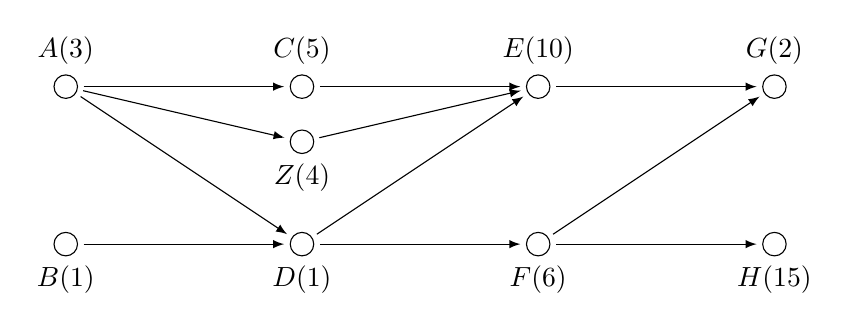
\begin{tikzpicture}[vtx/.style={draw, circle, inner sep = 3pt, font = \scriptsize}, myto/.style={-latex, shorten >=2pt, shorten <=2pt
}, node distance = \r cm]
\node[vtx, label=above:{$A(3)$}] (a) at (0,2){};
\node[vtx, label=below:{$B(1)$}] (b) at (0,0){};
\node[vtx, label=above:{$C(5)$}] (c) at (3,2){};
\node[vtx, label=below:{$D(1)$}] (d) at (3,0){};
\node[vtx, label=above:{ $E(10)$}] (e) at (6,2){};
\node[vtx, label=below:{$F(6)$}] (f) at (6,0){};
\node[vtx, label=above:{ $G(2)$}] (g) at (9,2){};
\node[vtx, label=below:{$H(15)$}] (h) at (9,0){};
\node[vtx, label=below:{$Z(4)$}] (z) at (3,1.3){};
\foreach \i/\j in {a/c,a/d,b/d,c/e,d/e,d/f,f/g,f/h,e/g,a/z,z/e}{\draw[myto] (\i) -- (\j);}
\end{tikzpicture}


\item Use your work above to answer the questions below.
	\begin{enumerate}
	\item Find a critical path and the critical time in the digraph above. What do you observe about the numbers you produced in the Backflow Algorithm?
	\vfill
	\item Determine the priority list using the Decreasing Time Algorithm.
	\vfill
	\item Determine the priority list by ordering the the vertices according to decreasing \emph{critical time}.
	\vfill
	\end{enumerate}
\newpage
\item In your own words, state the Critical Time Algorithm.
\vspace{.5in}
\item Use your two priority lists from the previous page to construct a schedule using two processors.\\
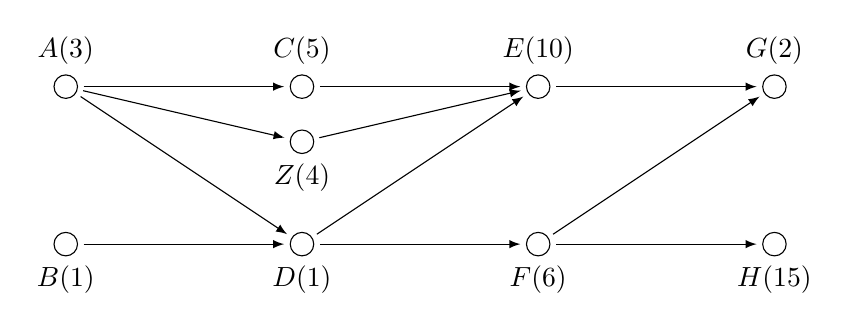
\begin{tikzpicture}[vtx/.style={draw, circle, inner sep = 3pt, font = \scriptsize}, myto/.style={-latex, shorten >=2pt, shorten <=2pt
}, node distance = \r cm]
\node[vtx, label=above:{$A(3)$}] (a) at (0,2){};
\node[vtx, label=below:{$B(1)$}] (b) at (0,0){};
\node[vtx, label=above:{$C(5)$}] (c) at (3,2){};
\node[vtx, label=below:{$D(1)$}] (d) at (3,0){};
\node[vtx, label=above:{ $E(10)$}] (e) at (6,2){};
\node[vtx, label=below:{$F(6)$}] (f) at (6,0){};
\node[vtx, label=above:{ $G(2)$}] (g) at (9,2){};
\node[vtx, label=below:{$H(15)$}] (h) at (9,0){};
\node[vtx, label=below:{$Z(4)$}] (z) at (3,1.3){};
\foreach \i/\j in {a/c,a/d,b/d,c/e,d/e,d/f,f/g,f/h,e/g,a/z,z/e}{\draw[myto] (\i) -- (\j);}
\end{tikzpicture}
	\begin{enumerate}
	\item decreasing time priority list: \underline{\hspace{2in}}\\
	
\hspace*{-1in}	\begin{tabular}{c || c}
time &   \quad \hspace{6in} \quad \\ \hline
done& \\ \hline
ready& \\ \hline
\end{tabular}

\vfill
	
	\hspace*{-1in}
	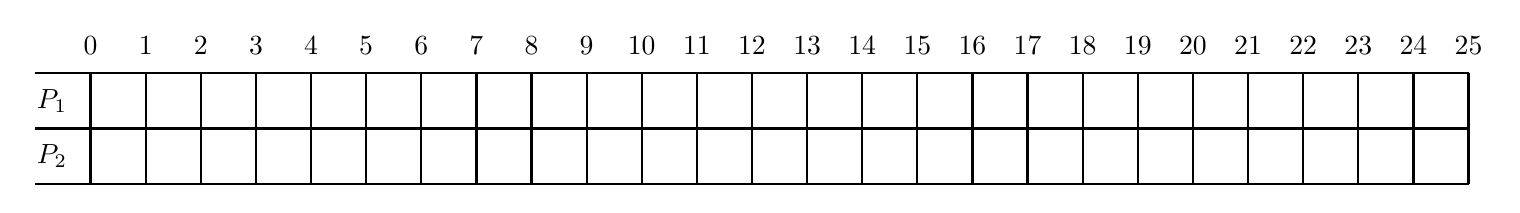
\begin{tikzpicture}[scale=.7]
\foreach \x in {0,1,...,25}{
	\node  at (\x,2.5){$\x$};
	\draw[thick] (\x,0) -- (\x,2);
	}
\foreach \y in {0,1,2}{\draw[thick] (-1,\y)--(25,\y);}
\node at (-.7,1.5){$P_1$};
\node at (-.7,.5){$P_2$};
\end{tikzpicture}
	\vfill
	\item decreasing \textbf{critical} time priority list: \underline{\hspace{2in}}\\
	
	\hspace*{-1in}	\begin{tabular}{c || c}
time &   \quad \hspace{6in} \quad \\ \hline
done& \\ \hline
ready& \\ \hline
\end{tabular}

\vfill
	
	\hspace*{-1in}
	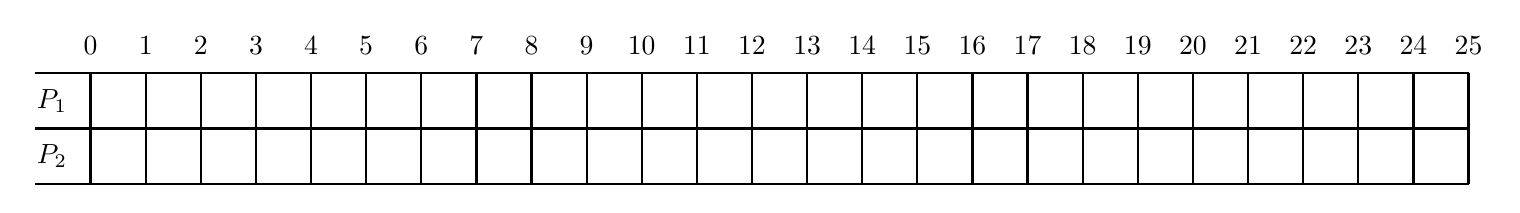
\begin{tikzpicture}[scale=.7]
\foreach \x in {0,1,...,25}{
	\node  at (\x,2.5){$\x$};
	\draw[thick] (\x,0) -- (\x,2);
	}
\foreach \y in {0,1,2}{\draw[thick] (-1,\y)--(25,\y);}
\node at (-.7,1.5){$P_1$};
\node at (-.7,.5){$P_2$};
\end{tikzpicture}
	\vfill
	\end{enumerate}
\end{enumerate}
\end{document}